\documentclass[letterpaper,12 pt,titlepage]{article}
 
\usepackage[utf8]{inputenc}
\usepackage[spanish]{babel}
\usepackage{color}
\usepackage{lmodern}
\usepackage{amssymb}
\usepackage{parskip}
\usepackage{xcolor}
\usepackage{multicol}
\usepackage{anysize}
\usepackage{enumerate}
\usepackage{url}
\usepackage{pdfpages}
\usepackage[hidelinks]{hyperref}
\usepackage{chngcntr}
\counterwithout{footnote}{section}
\usepackage{float}

%izq der arr ab
\marginsize{2.5 cm}{2.5 cm}{1 cm}{1 cm} 

\begin{document}
    \begin{titlepage}
        \centering
        
\includegraphics[width=0.15\textwidth]{img/escudo_fi_color.png}\par\vspace{1cm}
        {\scshape\LARGE Facultad de Ingeniería \par}
        \vspace{1cm}
        {\scshape\Large Estructura y Programación de Computadoras
        \par}
        \vspace{1cm}
        {\scshape\Large Grupo 2
        \par}
        \vspace{1.5cm}
        {\huge\bfseries Proyecto Nº2\par}
        \vspace{2cm}
        {\Large 
            Martínez Baeza José Alfonso\\
            Santana Sánchez María Yvette
        \par}
        \vfill
        {\large 03 de junio de 2020\par}
    \end{titlepage}

    \tableofcontents
    \newpage

    \section{Introducción}

    \subsection{Objetivo}
        Se requiere desarrollar un programa en lenguaje ensamblador para arquitectura Intel x86 que muestre una calculadora de manera gráfica en pantalla.

    \subsection{Descripción del problema}
        Para programar una calculadora con gráficos en lenguaje ensamblador es necesario utilizar algunas interrupciones para el modo en el que visualizamos los programas en Dosbox, también se hará uso de algunas macros y procedimientos del proyecto anterior para acelerar el desarrollo de esta calculadora, la dificultad de este proyecto radica en la división de la pantalla para saber en donde se ubica el cursor y donde efectúa el cliqueo, esto implica tener claro cuanto miden los botones utilizados y los espacios que tenemos dentro de la pantalla. 

        Utilizaremos un código base distinto al proporcionado por el profesor, el código fuente base puede encontrarse en el siguiente respositorio Github:
        
        \url{https://github.com/Raufoon/Simple-Calculator-Assembly-Language-.git}

    \subsection{Planteamiento del problema}

        Desarrollar un programa en lenguaje ensamblador para arquitectura Intel x86 que muestre una calculadora de manera gráfica en pantalla.
        
        \begin{center}
            \begin{minipage}{0.95\linewidth}
                \begin{itemize}
                    \item Números del 0 al 9
                    \item Botón suma (+)
                    \item Botón resta (-)
                    \item Botón multiplicación (*)
                    \item Botón cociente (/)
                    \item Botón residuo (\%)
                    \item Botón resultado (=)
                    \item Botón AC
                    \item Botón C
                \end{itemize}
            \end{minipage}
        \end{center}

        \textbf{Consideraciones:}
        
        \begin{center}
            \begin{minipage}{0.95\linewidth}
                \begin{itemize}
                    \item Los números deben estar en sistema decimal (dígitos de 0-9).
                    \item Los números deberán ser enteros sin signo.
                    \item Cada número introducido por el usuario puede ser de hasta 4 dígitos. El programa debe restringir que el usuario introduzca más números.
                \end{itemize}
            \end{minipage}
        \end{center}

    \section{Desarrollo}

    Para la realización de este proyecto nos apoyaremos del uso de macros y procedimientos dentro del lenguaje ensamblador para poder reducir el número de líneas de código, explicaremos a grandes rasgos el funcionamiento de dos interrupciones.
    
    \subsection{Interrupciones}
    Las interrupciones son un método del que disponen los dispositivos e incluso los procesos para hacer notar a la CPU la aparición de alguna circunstancia que requiera su intervención, esto con el fin de que los dispositivos puedan provocar que la CPU deje por el momento o la tarea que estaba realizando y haga la interrupción que se requiere.
        
    Las interrupciones que veremos son tres, aunque la gama de interrupciones es mucho más amplia.
    \subsubsection{int 21h}
    La interrupción 21h es una de las mas usadas e importantes para trabajar con el sistema operativo ya que llama o invoca todos los servicios de llamada función DOS, este compuesto por un grupo amplio de funciones, por ello solo mencionaremos la más usadas.

    \begin{center}
        \begin{minipage}{0.85\linewidth}
            \begin{description}
                \item[00h:] Terminación de Programa.
                \item[01h:] Entrada de caracteres con eco.
                \item[02h:] Salida de caracteres.
                \item[05h:] Salida de impresora.
                \item[06h:] E/S directa de consola.
                \item[08h:] Entrada de caracteres sin eco.
                \item[09h:] Salida de una cadena de caracteres.
            \end{description}
        \end{minipage}
    \end{center}
    
    No todas las funciones mencionadas se utilizarán en este proyecto, aunque es importante señalar que las funciones como 08h y 01h, es decir, lectura sin eco y con eco respectivamente, se utilizaron en el proyecto anterior.

    \subsubsection{int 33h} 
    
    Esta es posiblemente una de las interrupciones que mas usaremos dentro de este proyecto, pues esta la que implica el manejo del ratón, dentro de esta misma interrupción tenemos las siguientes funciones de mayor uso.

    \begin{center}
        \begin{minipage}{0.85\linewidth}
            \begin{description}
                \item[00h:] Inicializa el ratón.
                \item[01h:] Muestra el apuntador del ratón.
                \item[02h:] Oculta el apuntador del ratón.
                \item[03h:] Obtiene el estado del botón y la posición del ratón.
                \item[04h:] Establece la posición del apuntador.
                \item[05h:] Obtiene información del botón presionado del ratón.
                \item[06h:] Obtiene la información acerca de la liberación del botón
                \item[07h:] Fija limites horizontales para el apuntador.
                \item[08h:] Fija limites verticales para el apuntador.
                \item[09h:] Establece el tipo de apuntador gráfico.
                \item[0Ah:] Establece el tipo de apuntador en texto.
            \end{description}
        \end{minipage}
    \end{center}

    Las funciones señaladas son las que deberemos tener en cuenta para el siguiente trabajo, como curiosidad esta interrupción trabaja directamente con el registro AX y no el Ah que se usan en las operaciones.

    \subsubsection{int 10h} 
    
    Esta interrupción selecciona y activa el modo de video.

    \begin{center}
        \begin{minipage}{0.85\linewidth}
            \begin{description}
                \item[00h:] Asignar modo de video
                \item[01h:] Asignar tipo de cursor
                \item[02h:] Situar posición del cursor
                \item[03h:] Leer posición del cursor
                \item[08h:] Obtener atributo y carácter en el cursor
                \item[09h:] Escribir atributo y carácter en el cursor
                \item[0Ah:] Escribir únicamente carácter en el cursor
                \item[0Bh:] Asignar paleta de colores
                \item[0Ch:] Mostrar pixel grafico
            \end{description}
        \end{minipage}
    \end{center}

    En este caso se trabaja con el registro AH, como vemos ya tenemos señalado las funciones que se mostraran mas adelante en el proyecto.

    \subsection{Código}
    \begin{center}
        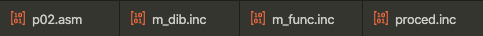
\includegraphics[width=0.9\textwidth]{img/01.png}
    \end{center}
    Como podemos notar en la imagen anterior tenemos el proyecto divido en tres archivos: p02, m\_dib, m\_func y proced, esto con el fin de separar el código para una cómoda lectura no solo de un tercero sino de nosotros mismos para descubrir posibles errores de manera más rápida.

    \begin{center}
        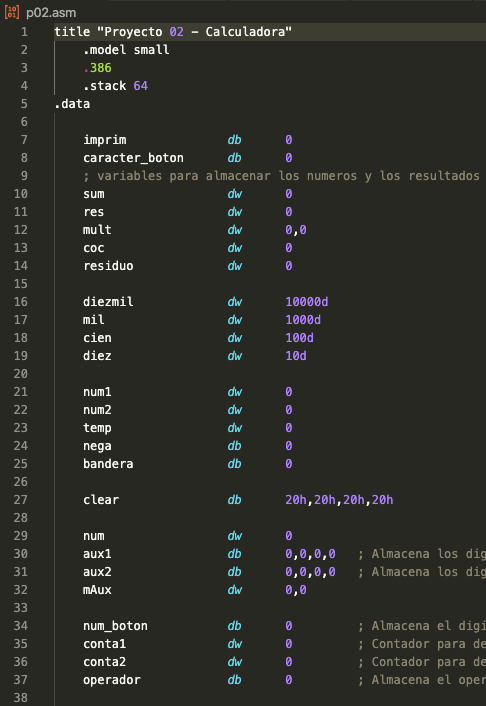
\includegraphics[width=0.42\textwidth]{img/02.png}
        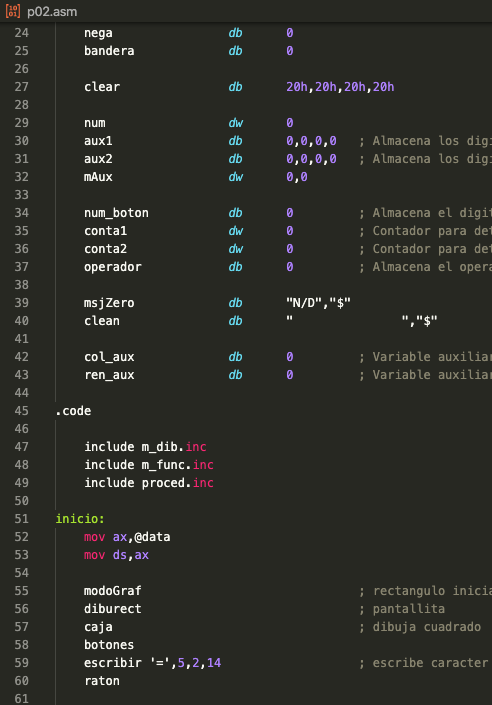
\includegraphics[width=0.42\textwidth]{img/03.png}
    \end{center}

    Tenemos las directivas conocidas en el proyecto anterior, en .data se ubican las variables que vamos a utilizar a lo largo del código, aux1 y aux2 será la variable que guarde los 4 dígitos que se van a introducir por medio del ratón, en .code podemos ver como incluimos dentro del archivo p02.asm los otros componentes (o podemos verlos como bibliotecas locales semejante a C), donde m\_dib y m\_func contienen las respectivas macros utilizadas dentro del código para hacer el tema grafico mientras que proced contiene procedimientos que acumulan los cuatro dígitos en una variable para luego imprimirla (adaptación del proyecto anterior).

    \begin{center}
        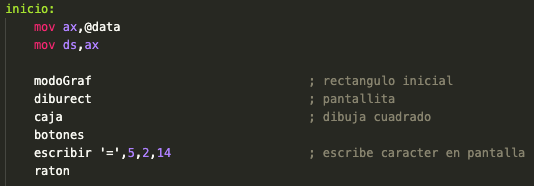
\includegraphics[width=0.9\textwidth]{img/04.png}
    \end{center}
    
    Dentro de la etiqueta inicio, que pertenece a la directiva .code, podemos ver como comenzamos el programa, con su respectiva reserva de segmento, posteriormente se hace una llamada a las macros en este caso modoGraf,diburect, caja, botones y ratón.
    
    A continuación, analizaremos dichas macros (iremos por ello al apartado m\_dib.inc) al bloque de código perteneciente a modoGraf.

    \begin{center}
        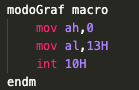
\includegraphics[width=0.3\textwidth]{img/05.png}
    \end{center}

    Imaginemos que solo tenemos el código anterior ejecutado en el inicio, entonces al ejecutarlo en DOSBox encontraremos los siguiente:

    \begin{figure}[H]
    \centering
    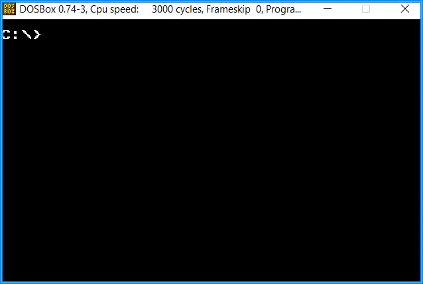
\includegraphics[width=0.55\textwidth]{img/06.png}
    \caption{Entra en modo gráfico}
    \end{figure}

    Con este apartado de código iniciamos el modo grafico con la interrupción 13h.
    
    En la siguiente imagen veremos las macros de diburect, caja.
    
    \subsubsection{Interfaz gráfica}

    \begin{center}
        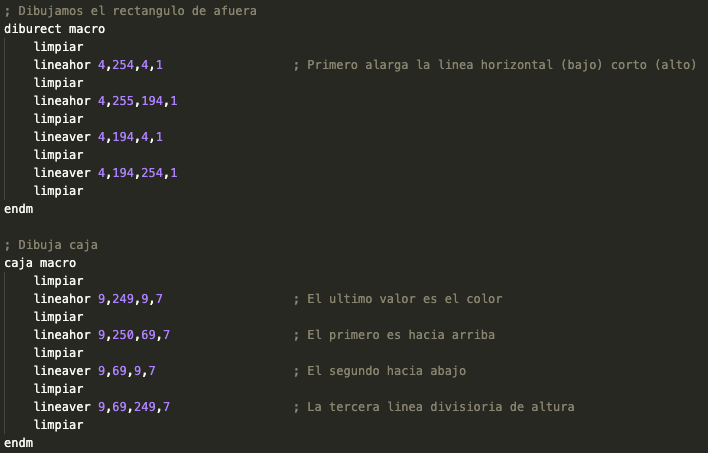
\includegraphics[width=0.9\textwidth]{img/07.png}
    \end{center}

    En diburect, primero limpia la pantalla, posteriormente genera dos líneas horizontales y otras dos líneas verticales.

    Nuevamente para ejemplificar mejor el desarrollo de este programa, mostraremos paso a paso como se desarrolla la transformación gráfica.
    
    En la macro tenemos la siguiente línea de código:

    \begin{itemize}
        \item lineahor \textcolor{blue}{4},\textcolor{red}{254},\textcolor{green}{4},1 
        \begin{center}
            \begin{minipage}{0.85\linewidth}
                \begin{description}
                    \item[\textcolor{blue}{Parámetro 1:}] La extensión de la línea horizontal hacia la izquierda.
                    \item[\textcolor{red}{Parámetro 2:}] La extensión de la línea horizontal hacia la derecha.
                    \item[\textcolor{green}{Parámetro 3:}] La posición de la línea horizontal más arriba o abajo.
                    \item[Parámetro 4:] Determina el color.
                \end{description}
            \end{minipage}
        \end{center}

        \item lineaver \textcolor{blue}{4},\textcolor{red}{254},\textcolor{green}{4},1 
        \begin{center}
            \begin{minipage}{0.85\linewidth}
                \begin{description}
                    \item[\textcolor{blue}{Parámetro 1:}] La extensión de la línea vertical hacia la izquierda.
                    \item[\textcolor{red}{Parámetro 2:}] La extensión de la línea vertical hacia la derecha.
                    \item[\textcolor{green}{Parámetro 3:}] La posición de la línea vertical más arriba o abajo.
                    \item[Parámetro 4:] Determina el color.
                \end{description}
            \end{minipage}
        \end{center}
    \end{itemize}
    
    Estos códigos llaman a su vez a otra macro que determina el dibujo del rectángulo.

    \begin{center}
        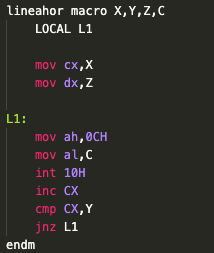
\includegraphics[width=0.45\textwidth]{img/08.png}
        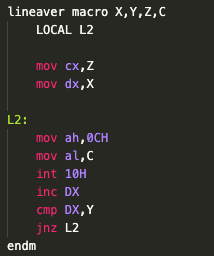
\includegraphics[width=0.45\textwidth]{img/09.png}
    \end{center}

    \begin{figure}[H]
    \centering
    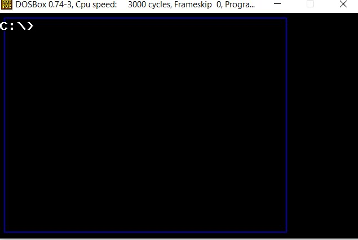
\includegraphics[width=0.8\textwidth]{img/10.png}
    \caption{Dibuja marco de la calculadora}
    \end{figure}

    Al agregar la macro caja al código dibujaremos nuevamente otro rectángulo valiéndonos de las macros utilizadas anteriormente líneahor y lineaver.

    \begin{figure}[H]
    \centering
    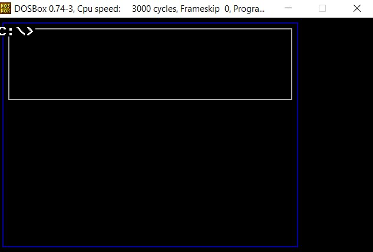
\includegraphics[width=0.8\textwidth]{img/11.png}
    \caption{Dibuja caja donde imprimirá las operaciones}
    \end{figure}

    Un detalle importante al dibujar los rectángulos que deseamos debemos siempre tener en cuenta que ese código debe ir después de ejecutar el modo gráfico, sino el dibujo no se realizará.

    \begin{center}
        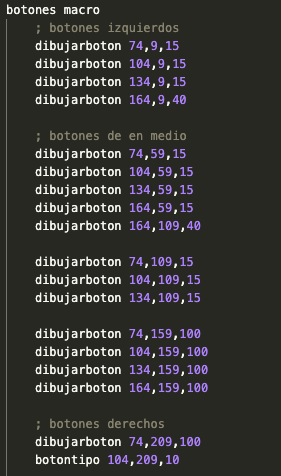
\includegraphics[width=0.4\textwidth]{img/12.png}
        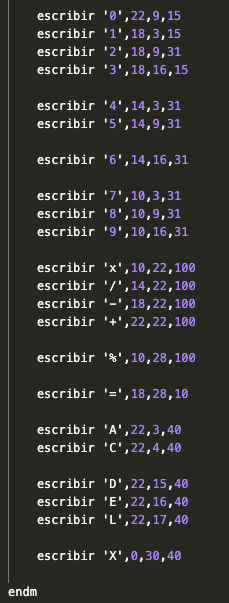
\includegraphics[width=0.25\textwidth]{img/13.png}
    \end{center}

    En esta línea de código se invocan dos macros:
    \begin{itemize}
        \item escribir \textcolor{blue}{`0'},\textcolor{red}{22},\textcolor{green}{9},15 
        \begin{center}
            \begin{minipage}{0.85\linewidth}
                \begin{description}
                    \item[\textcolor{blue}{Parámetro 1:}] Se envía el carácter que deseamos imprimir dentro del modo gráfico.
                    \item[\textcolor{red}{Parámetro 2:}] Posiciona el carácter hacia arriba o abajo.
                    \item[\textcolor{green}{Parámetro 3:}] Posiciona el carácter hacia la derecha o izquierda
                    \item[Parámetro 4:] Determina el color del caracter.
                \end{description}
            \end{minipage}
        \end{center}

        \item dibujarboton  \textcolor{blue}{74},\textcolor{red}{9},\textcolor{green}{15}
        \begin{center}
            \begin{minipage}{0.85\linewidth}
                \begin{description}
                    \item[\textcolor{blue}{Parámetro 1:}] Posiciona el botón hacia arriba o abajo.
                    \item[\textcolor{red}{Parámetro 2:}] Posiciona el botón hacia la derecha o hacia la izquierda.
                    \item[\textcolor{green}{Parámetro 3:}] Determina el color del botón.
                \end{description}
            \end{minipage}
        \end{center}
    \end{itemize}

    La imagen siguiente muestra como se ve lo anteriormente mencionado para una mejor visualización de lo explicado.

    \begin{figure}[H]
    \centering
    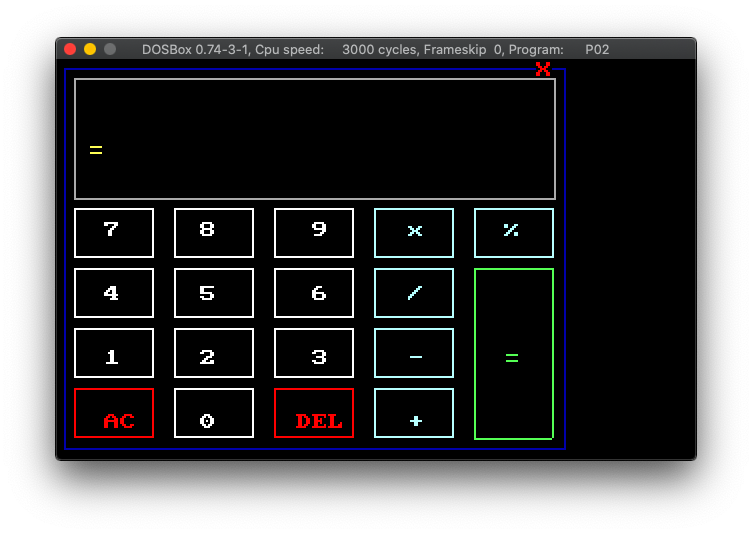
\includegraphics[width=0.8\textwidth]{img/14.png}
    \caption{Dibuja botones}
    \end{figure}

    En la macro de botones debemos analizar la macro dibujarboton, botontipo y escribir, ya que esta dibuja las letras dentro de los botones.

    \begin{center}
        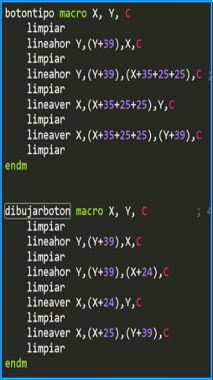
\includegraphics[width=0.45\textwidth]{img/15.png}
        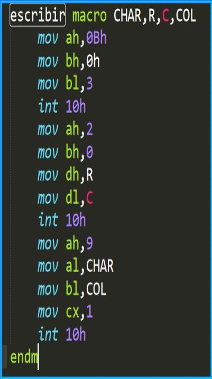
\includegraphics[width=0.45\textwidth]{img/16.png}
    \end{center}

    Estas macros anteriores son las encargadas de dibujar el botón y los caracteres que los representa para el usuario.

    Otra de las macros importante es la ratón es la encargada de inicializar el mouse y mostrarlo.

    \begin{center}
        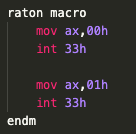
\includegraphics[width=0.3\textwidth]{img/17.png}
    \end{center}

    \subsubsection{Funcionamiento lógico}

    Una vez que se tiene la interfaz gráfica dibujada es necesario programar el código necesario para hacer funcionar cada uno de los botones, para esto es necesario ir delimitando la zona de cada botón en donde permitirá dar clic.

    Al iniciar se verifica si se presiona el boton izquierdo del mouse, una vez que se comprueba esto se compara con el número de columna, si es menor o igual a $48$ es probable que se haya presionado sobre los botones más a la izquierda (7,4,1 o AC); si es menor o igual a $98$ es probable que se haya presionado sobre los números del centro (8,5,2 o 0); si es menor o igual a $148$ es probable que se haya presionado sobre los números más a la derecha (9,6,3 o DEL); si es menor o igual a $198$ es probable que se haya presionado sobre los botones de operaciones (X,/,$-$ o $+$) y si es menor o igual a $198$ es probable que se haya presionado sobre los botones más a la derecha (\% o $=$)

    \begin{center}
        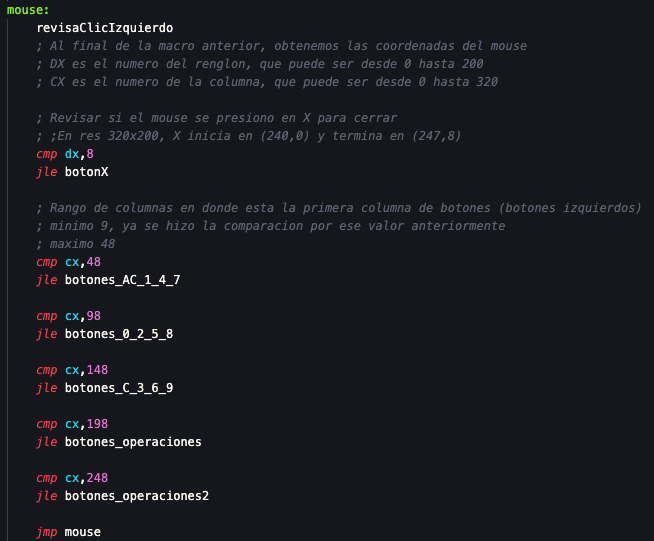
\includegraphics[width=0.8\textwidth]{img/18.png}
    \end{center}


    El código base proporcionado por el profesor sugería una triple comprobación para verificar que estuviera dentro del rango de botones, dentro de ciertas columnas y dentro de ciertos renglones, parecía una solución viable, sin embargo al avanzar con el desarrollo del proyecto nos dimos cuenta de que el código comenzaba a extenderse demasiado, por lo que decidimos reducir estas comprobaciones con una macro llamada $isButton$ la cual recibe 4 parámetros:
    $xmin$, $xmax$, $ymin$ y $ymax$, estos hacen referencia a las cuatro esquinas que conforman un boton y a su vez su funcionamiento puede extenderse para verificar una zona completa.

    \begin{center}
        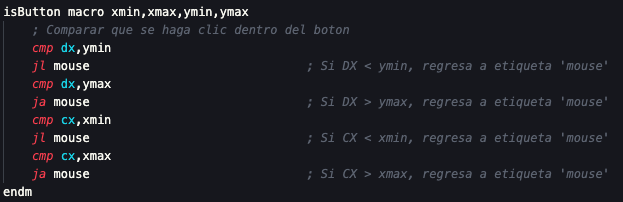
\includegraphics[width=0.8\textwidth]{img/19.png}
    \end{center}

    Una vez que se comprueba que se hace clic sobre un botón se realizan distintas operaciones dependiendo del tipo de botón del cual se trate.

    Si es un \textbf{número} se almacena el valor correspondiente en la variable \textit{num\_boton} y da el salto a la etiqueta \textit{lee\_num1}

    \begin{center}
        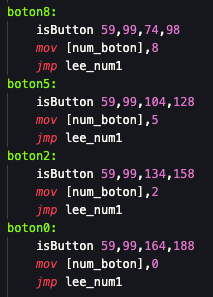
\includegraphics[width=0.6\textwidth]{img/20.png}
        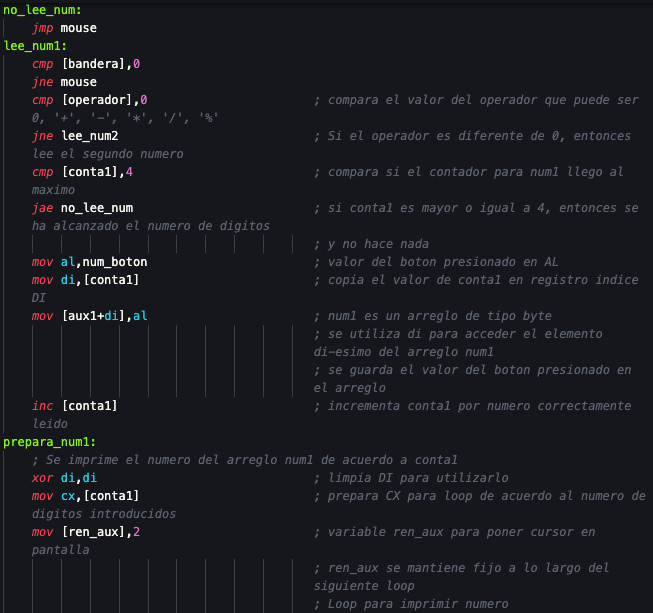
\includegraphics[width=0.85\textwidth]{img/20-1.png}
        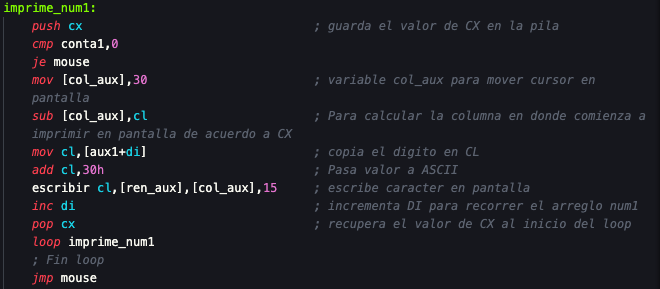
\includegraphics[width=0.85\textwidth]{img/20-2.png}
    \end{center}

    Esta parte del código se encarga de almacenar el dígito almacenado en la variable \textit{num\_boton} en un arreglo de 4 elementos tipo Byte e imprimirlos en pantalla recorriendo el arreglo con ayuda del registro \textit{di}. Tambíen se encarga de comprobar si ingresamos por lo menos un dígito para no permitir al usuario efectuar operaciones sin números, comprueba si estamos ingresando dígitos para el primer o segundo número o si el resultado ya se muestra en pantalla para no cambiar los números sin limpiar antes a pantalla.

    \begin{figure}[H]
    \centering
    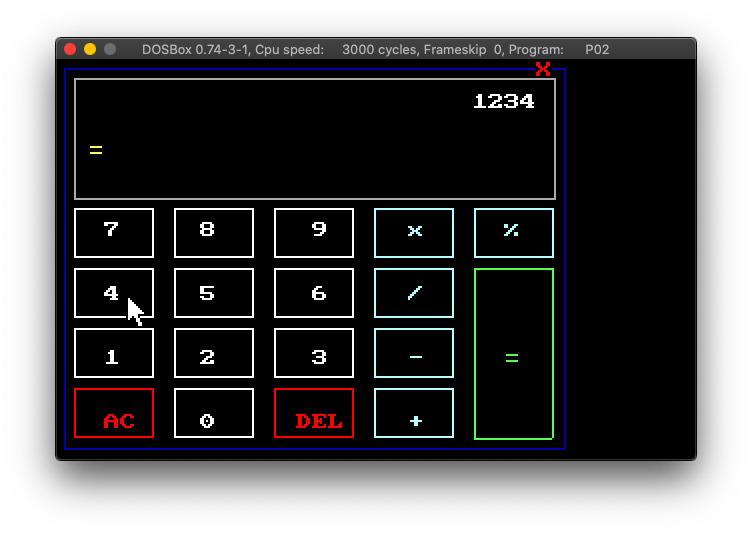
\includegraphics[width=0.65\textwidth]{img/21.png}
    \caption{Lee e imprime digitos del primer número.}
    \end{figure}

    Si el botón fuera de operación entonces se verifica que se haya ingresado por lo menos un número comprobando \textit{conta1} con $0$, si es igual entonces no permite ingresar ningún símbolo y si es distinto de $0$ (o en este caso mayor), guarda el respectivo símbolo en la variable \textit{operador} y lo pinta en pantalla con un color amarillo un renglón abajo del primer número y completamente a la izquierda.

    \begin{center}
        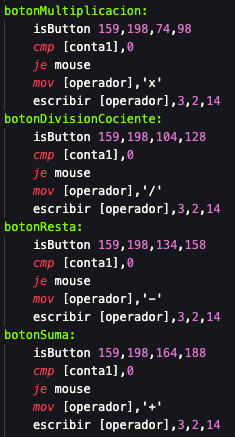
\includegraphics[width=0.37\textwidth]{img/22.png}
    \end{center}

    \begin{figure}[H]
    \centering
    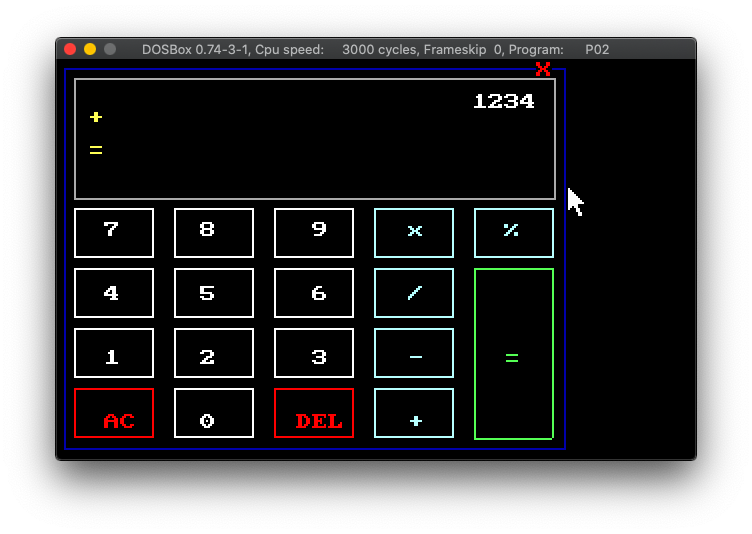
\includegraphics[width=0.7\textwidth]{img/23.png}
    \caption{Imprime símbolo de la operación aritmética a realizar.}
    \end{figure}

    Para el segundo número se comprueba si la variable \textit{operador} es distinto de cero, para este punto esta comprobación será verdadera por lo que comenzaremos a almacenar dígitos en un segundo arreglo para posteriormente imprimir el segundo número 2 renglones más abajo del primero.

    Fuera de esto las operaciones realizadas son las mismas que para el primer número.

    Cabe aclarar que para ambos números el programa deja de leer dígitos cuando el respectivo contador (\textit{conta1} o \textit{conta2}) llegue a 4.

    \begin{figure}[H]
    \centering
    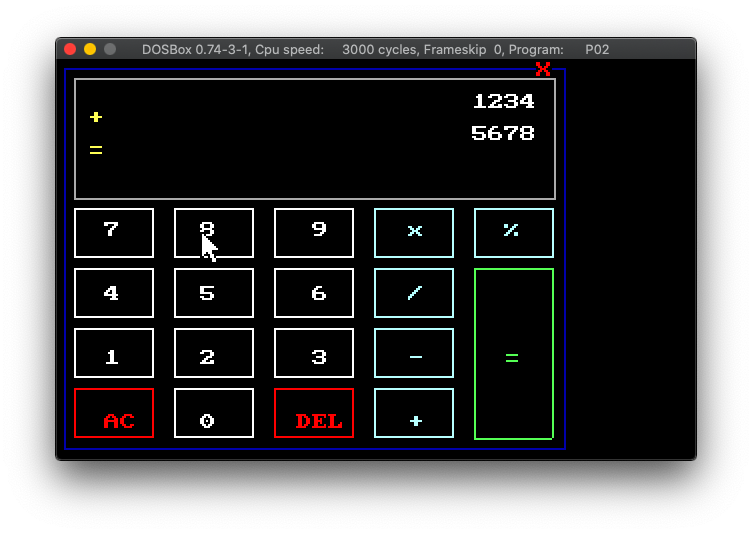
\includegraphics[width=0.7\textwidth]{img/24.png}
    \caption{Lee e imprime dígitos del segundo número.}
    \end{figure}

    El siguiente botón es el de resultado, este botón podría decirse que contiene la lógica más importante del programa debido a que es aquí donde se procesan los dígitos previamente almacenados en arreglo y a su vez hace llamado de las procedimientos y macros que se encargan de realizar e imprimir las operaciones.

    \begin{center}
        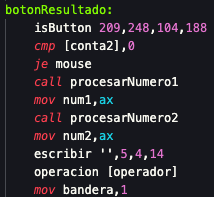
\includegraphics[width=0.4\textwidth]{img/25.png}
    \end{center}

    Los procedimientos \textit{procesarNum1} y \textit{procesarNum2} fueron reutilizados del proyecto anterior pero adaptados de tal manera que utilizaran los valores almacenados en un arreglo a diferencia de las variables independientes dedicadas a almacenar unidades, decenas, centenas o millares.

    \begin{center}
        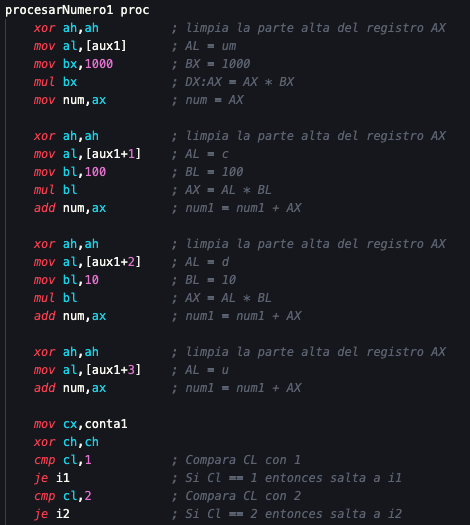
\includegraphics[width=0.45\textwidth]{img/26.png}
        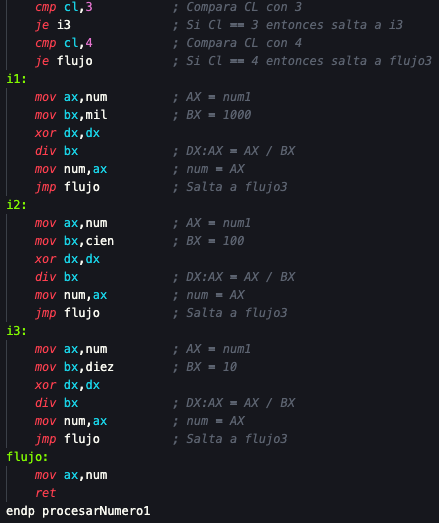
\includegraphics[width=0.42\textwidth]{img/27.png}
    \end{center}

    Posteriormente es necesario posicionar el cursor al final del signo $=$, esto para poder imprimir el resultado reutilizando el código del proyecto anterior utilizando la interrupción $21h$ descrita con anterioridad. 

    Para realizar la operación deseada hacemos uso de la macro \textit{operacion} pasando como parámetro a \textit{operador}. Una diferencia importante con respecto al proyecto anterior es que esta calculadora no requiere de realizar todos las operaciones por cada ejecución, por lo que implementamos un salto al final de cada operación para salir de este procedimiento. 
    
    Independientemente a los cambios mencionados y junto con la usencia de mensajes en pantalla, la implementación de las operaciones aritméticas del proyecto anterior es la misma.

    Al final se cambia el valor de la variable \textit{bandera} a $1$ para indicar que el resultado ya se muestra en pantalla, esto nos servirá para cambiar ligeramente el funcionamiento del botón \textit{DEL} para que se comporte igual que \textit{AC} los cuales se explicarán más adelante.

    \begin{figure}[H]
    \centering
    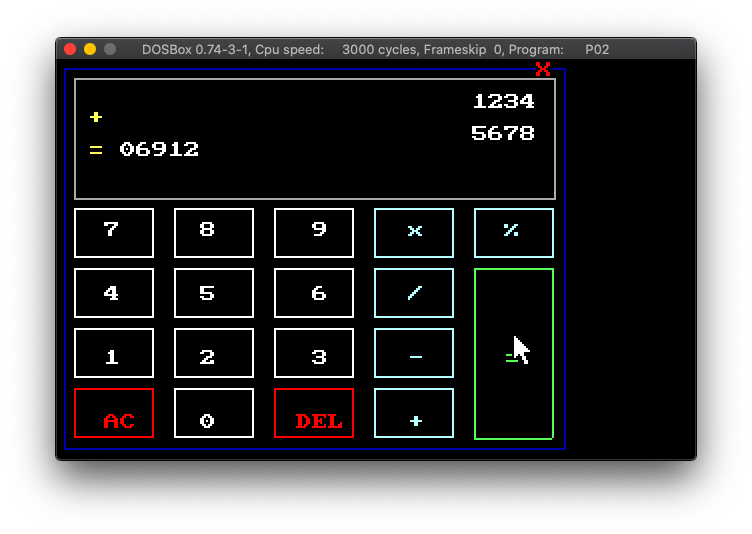
\includegraphics[width=0.7\textwidth]{img/28.png}
    \caption{Imprime el resultado de la operación realizada.}
    \end{figure}

    Otro tipo de botones, como hemos podido ver, son los diseñados para borrar, ya sea dígito por dígito (\textit{DEL}) o toda la pantalla al mismo tiempo (\textit{AC}).

    La implementación de estos botones parecía sencilla durante el planteamiento, sin embargo, fue una de la que más nos costó trabajo al momento de afinar detalles pues en nuestras primeras pruebas los dígitos parecían borrarse pero dejaba remanentes en pantalla al continuar escribiendo, es decir, si por ejemplo escribíamos $1234$ y borrábamos dos dígitos ($12\_\_$) porque realmente queríamos escribir $128$ había un error de impresión por el cual se pintaba en pantalla el número $1128$, sin embargo el resultado se imprimía correctamente utilizando como operandos los números deseados, que para este ejemplo es $128$.

    Así mismo, una primera solución para el botón AC era dar un salto a la etiqueta \textit{inicio} no sin antes inicializar las variables en $0$'s, pero estéticamente no era de nuestro agrado, pues generaba un parpadeo en la pantalla, es por esto que decidimos aplicar un método un poco ``\textit{arcaico}'' (por decirlo de alguna manera) que consiste en declarar un mensaje de 8 espacios en blanco e imprimirlos en la misma posición donde estaba la impresión del resultado y un arreglo de 4 espacios para sobreescribir los operandos.

    \begin{center}
        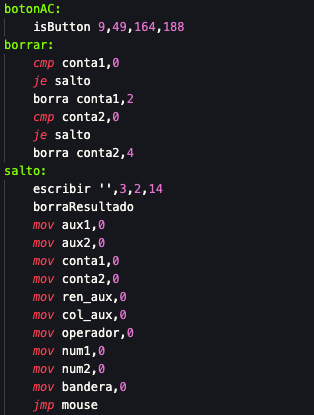
\includegraphics[width=0.45\textwidth]{img/29.png}
        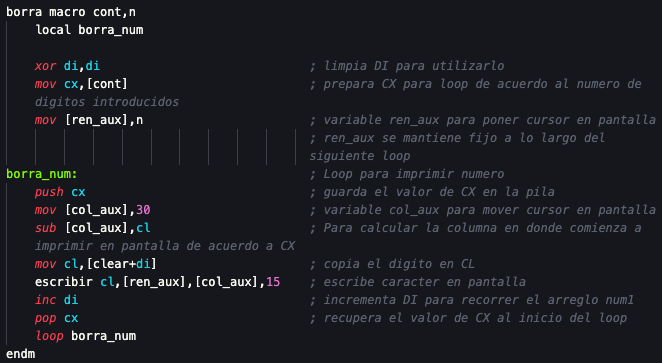
\includegraphics[width=0.9\textwidth]{img/30.png}
    \end{center}

    Una vez que se detecta el botón, se compara si el contador del primero número es $0$, si es asi entonces no borra nada y solo inicializa variables en caso de ser mayor a $0$ entonces imprime el arreglo de espacios segun la cantidad de dígitos que haya guardado, todo esto con ayuda del registro $di$. Lo mismo sucede para el segundo número. Y para el resultado imprime un mensaje de 8 espacios debido a que es la cantidad máxima de dígitos que puede mostrar el resultado.

    \begin{center}
        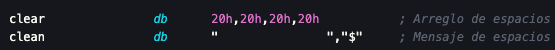
\includegraphics[width=0.9\textwidth]{img/31.png}
        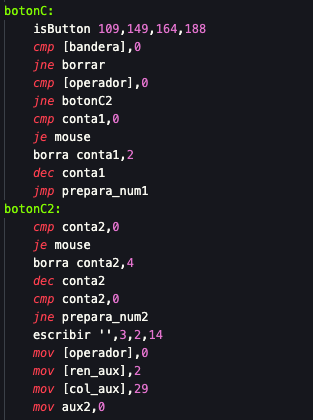
\includegraphics[width=0.65\textwidth]{img/32.png}
    \end{center}

    Para el botón \textit{DEL}, primero se compara la \textit{bandera} con $0$, pues de ser diferente de 0 el funcionamiento de este botón es idéntico al de \textit{AC}, es decir, borra la pantalla.

    De lo contrario, se compara ahora el estado del \textit{operador}, ya que este nos indica cuál de los dos número es el que se está modificando.

    Si resulta ser $0$ el valor de ambas comparaciones entonces se procede a eliminar el último dígito del primer número.

    Si en la segunda comparación \textit{operador} contiene un valor diferente de $0$, entonces se elimina el último dígito del segundo número.

    En el proceso de borrado de dígitos del segundo número, cuando el contador llega a $0$ también de borra de la pantalla el símbolo del operando.

    \section{Diagramas de flujo}
    \begin{center} 
        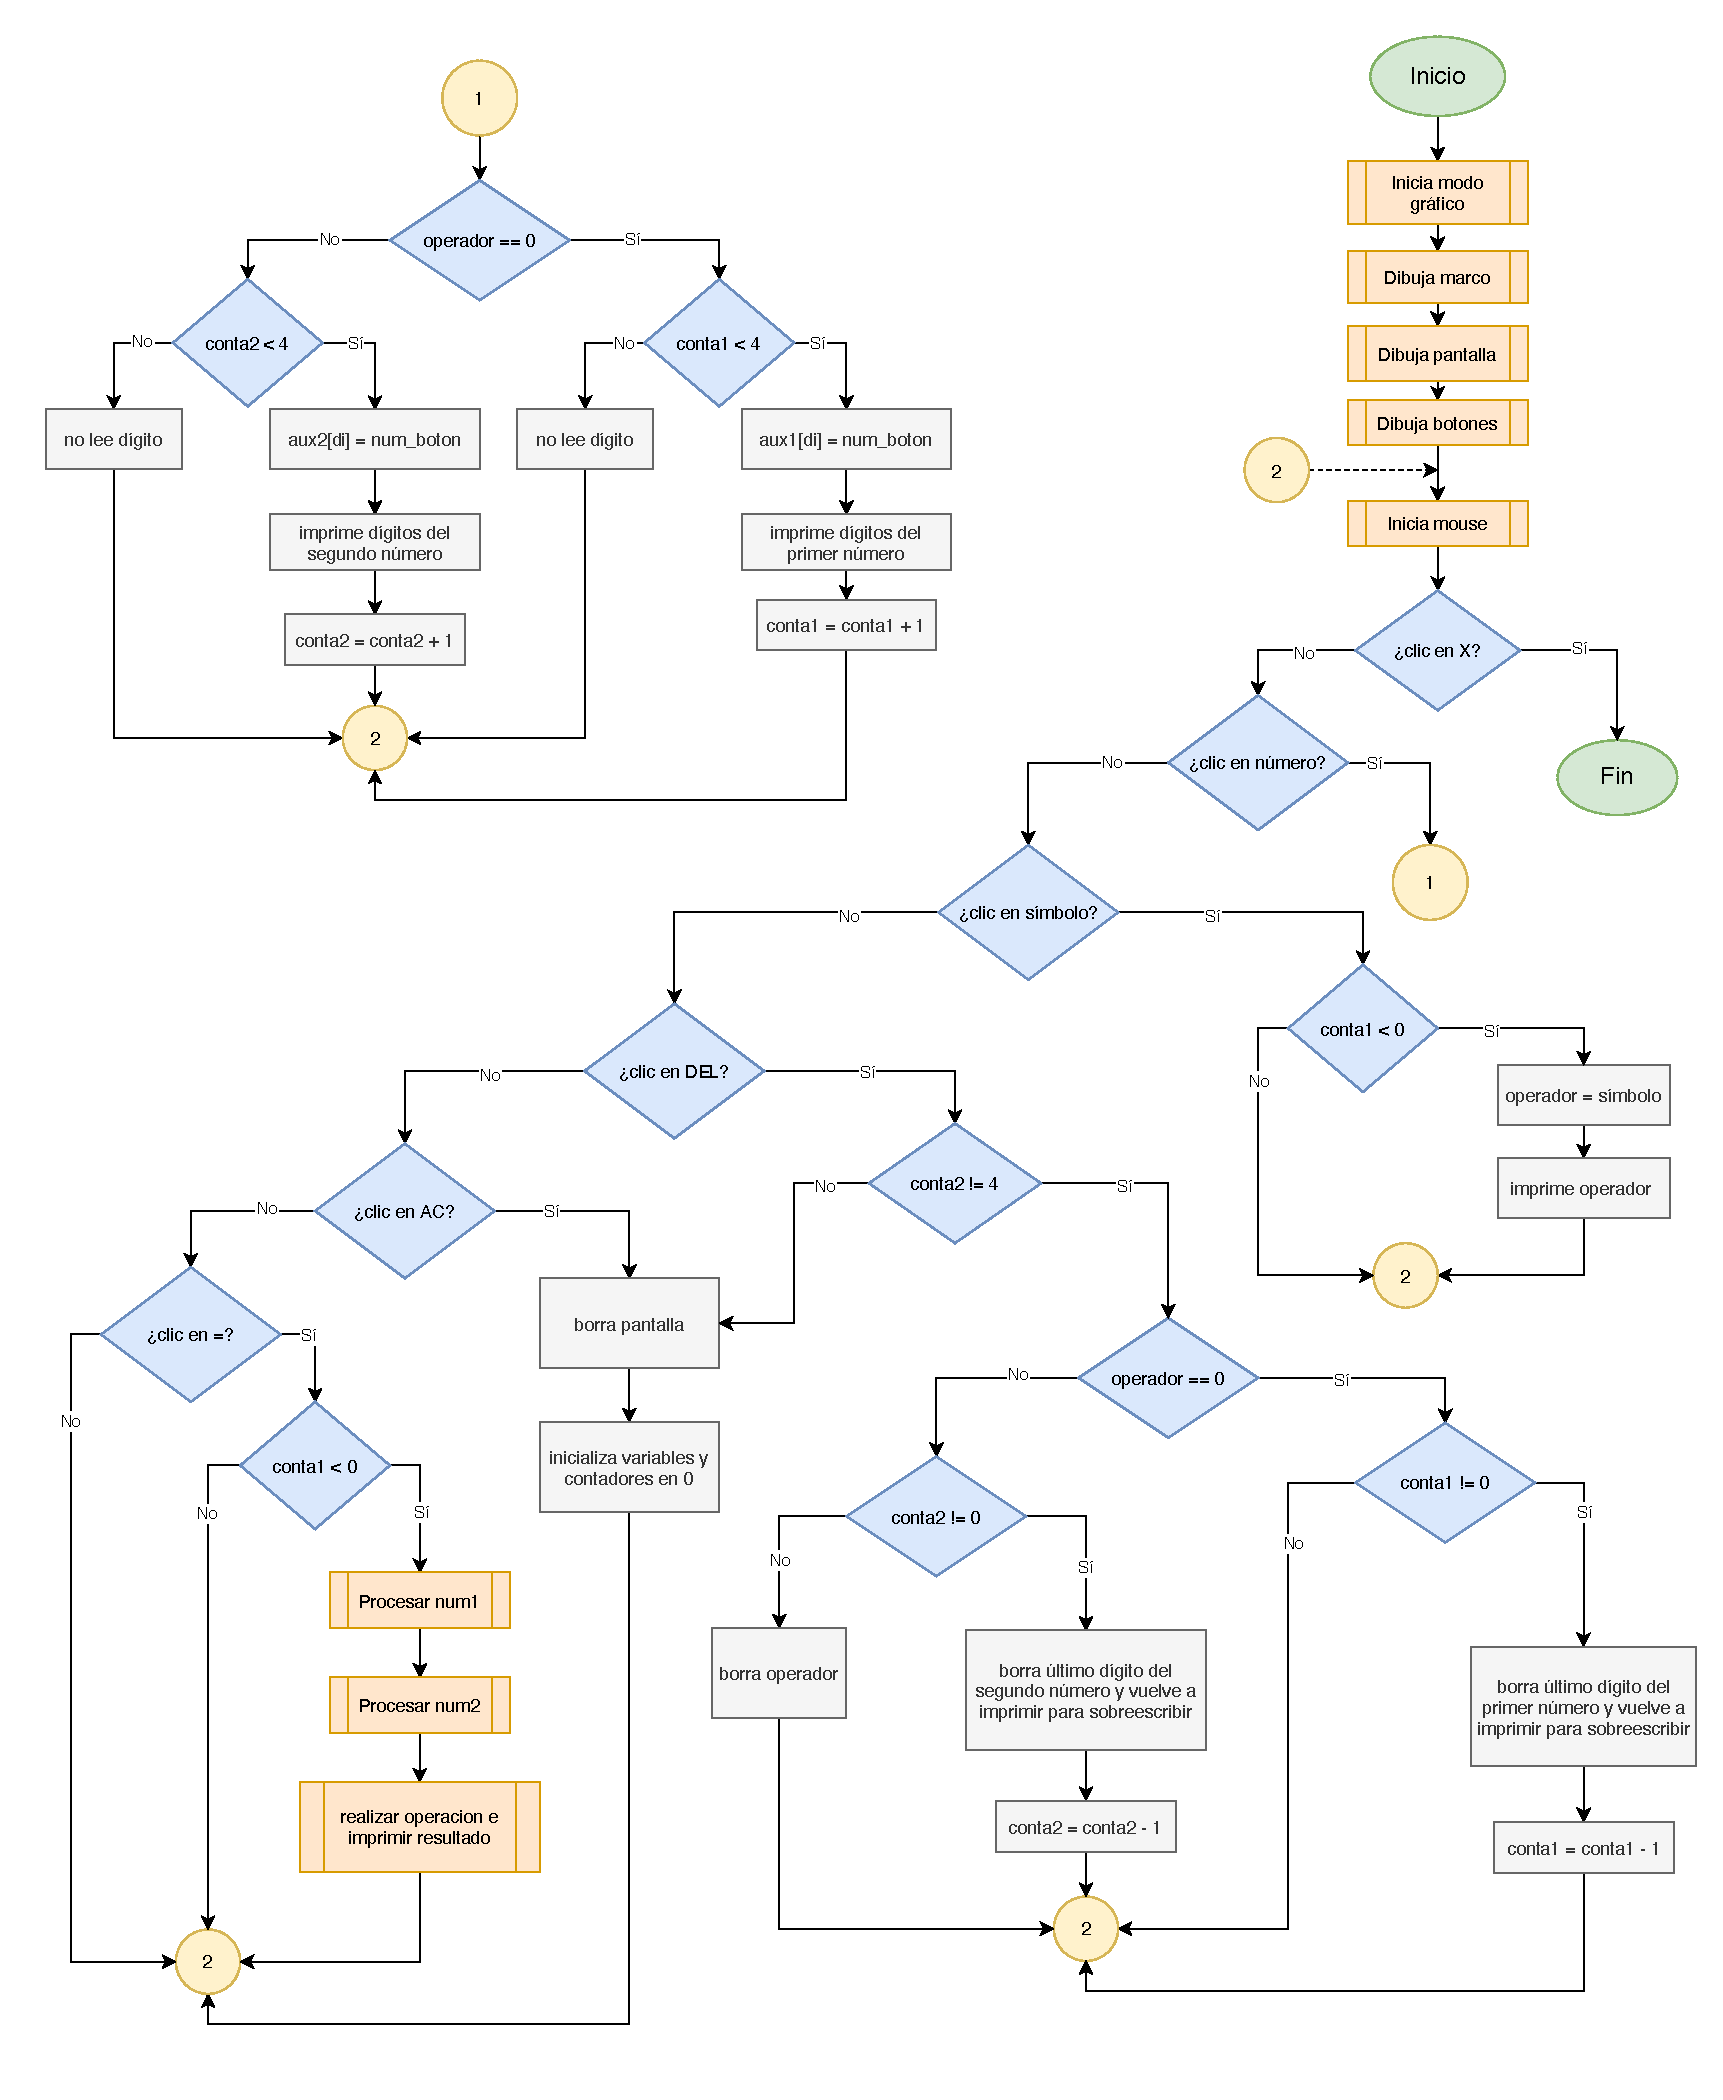
\includegraphics[width=1\textwidth]{img/diagramas/p02.pdf}

        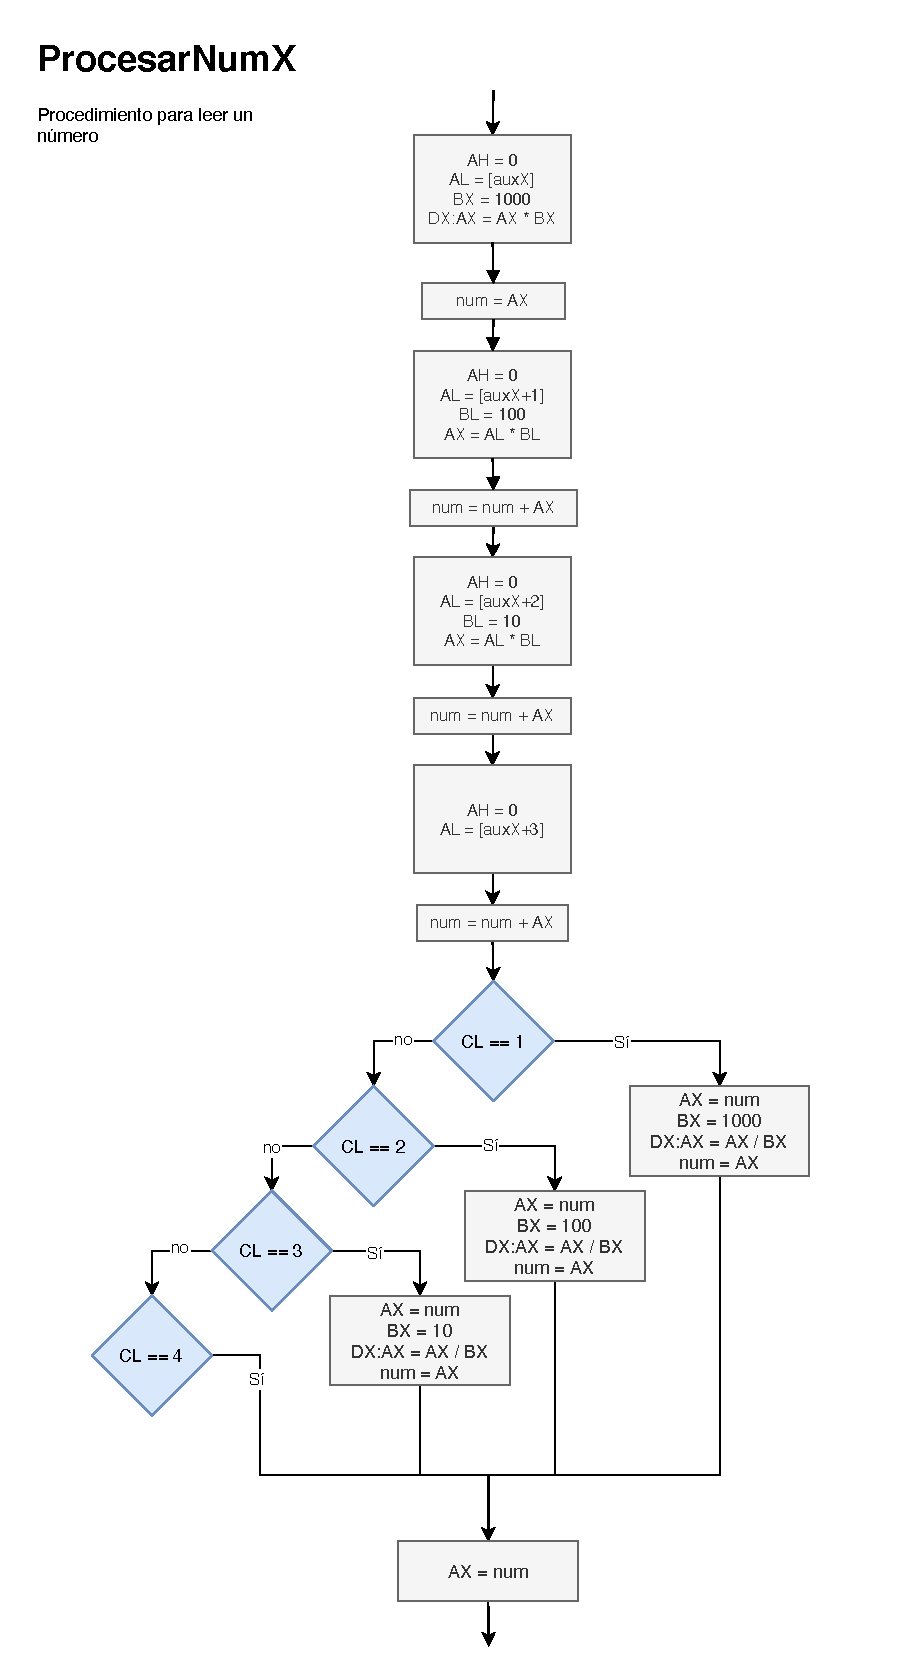
\includegraphics[width=0.73\textwidth]{img/diagramas/p01-ProcNum.pdf}

        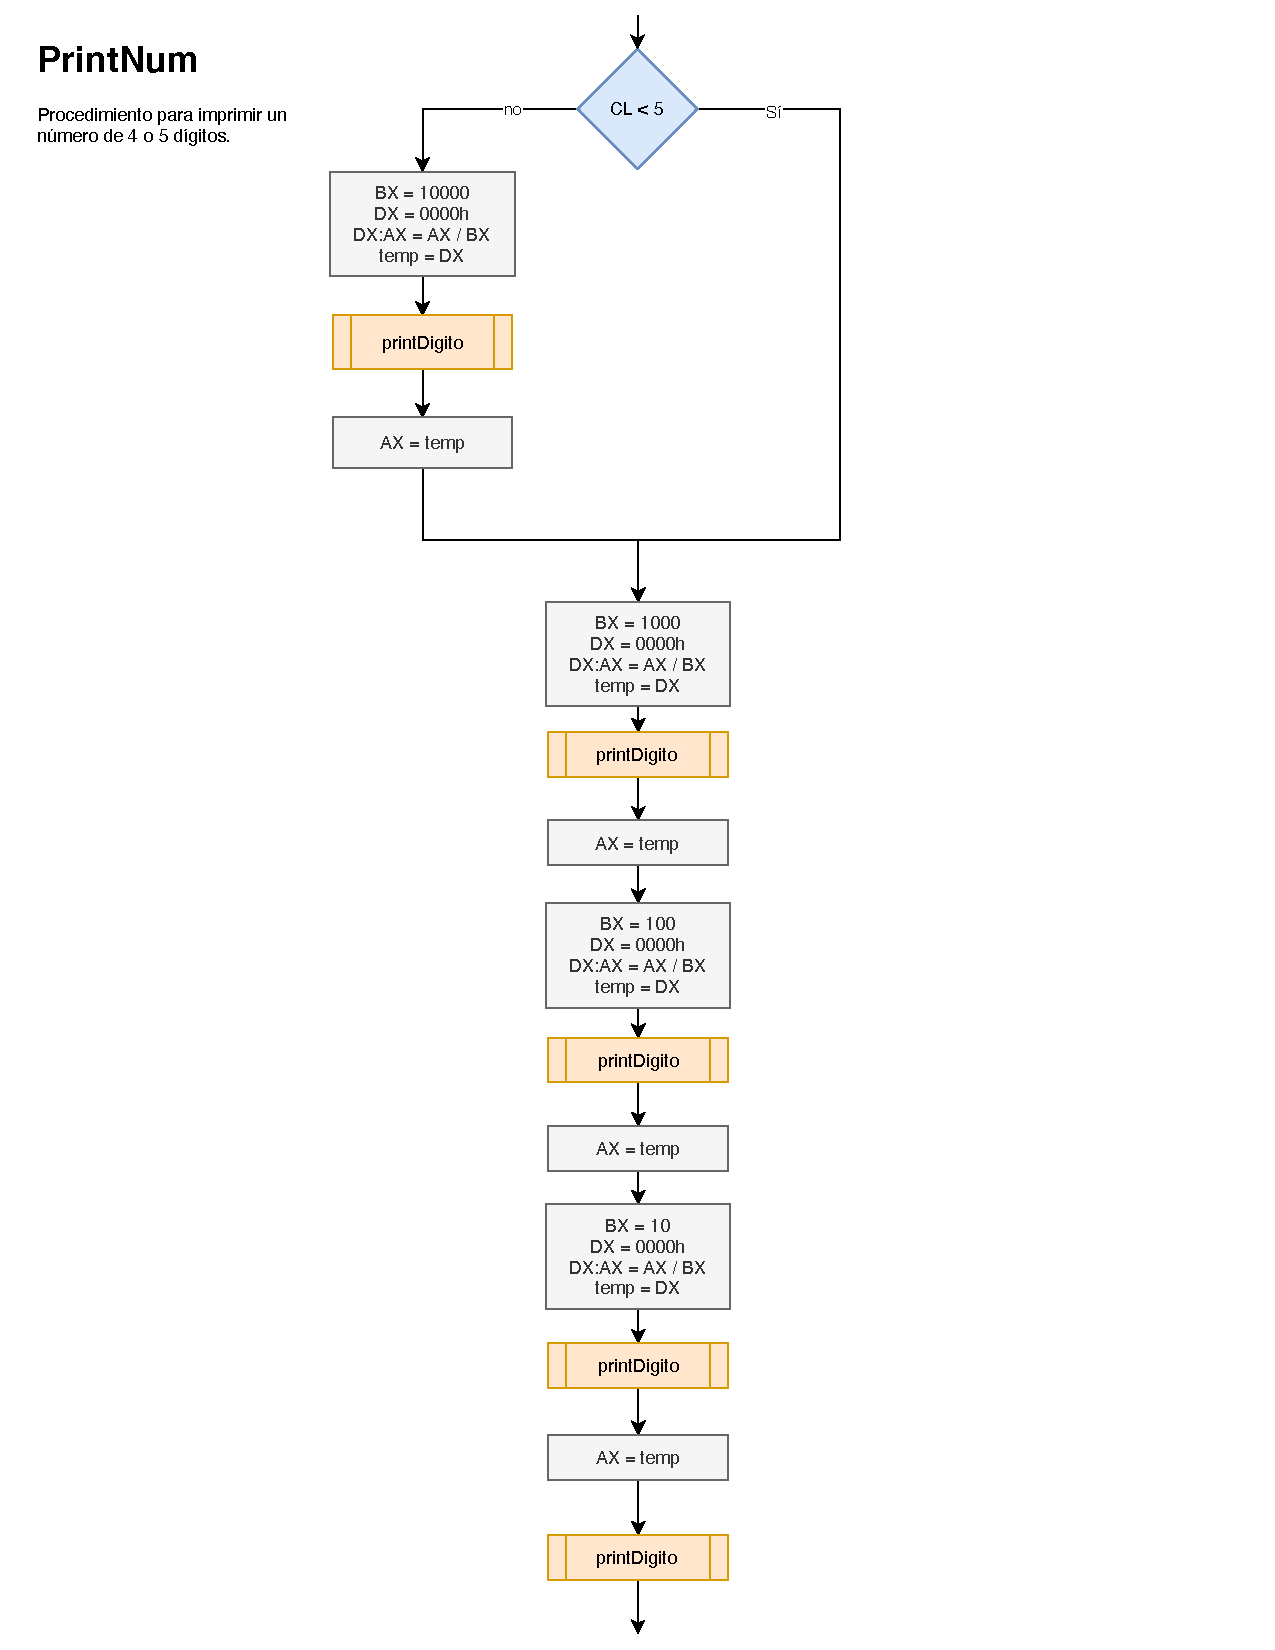
\includegraphics[width=1\textwidth]{img/diagramas/p01-PrintNum.pdf}
    \end{center}

    \section{Pruebas de escritorio}
    \section{Conclusiones}

\end{document}





